\documentclass[11pt, oneside]{article}

\usepackage{graphicx}
\usepackage{amssymb}
\usepackage{multirow}
\usepackage{float}
\usepackage{amsthm}
\usepackage[left=2cm, right=2cm, top=2cm]{geometry}
\usepackage{array}
\usepackage{pstricks-add}


\theoremstyle{definition}
\newtheorem{exmp}{Example}[section]

\def\rot{\rotatebox}

\begin{document}

\section{What are Natural Numbers?}

Natural Numbers are the first type of numbers that were used historically and are the numbers that are used for counting, which is why they are sometimes called Counting Numbers. The first known use of written numbers is from a carving in bones from approximately 150,000 years ago, which is thought to be used to count and can be seen in the following picture:

\begin{figure}[ht!]
\centering
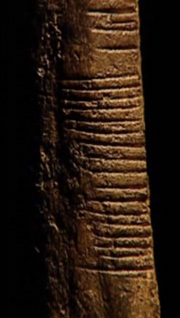
\includegraphics[width=60mm]{bone-carving.jpg}
\caption{Bone carvings used for counting \label{overflow}}
\end{figure}

Numbers evolved and number systems were defined in order to be able to use them more easily and the number system that we use now, which has its origin in India, became the standard system. We also use other numerical systems, for example when counting time, which we will study later on. 

\subsection{Place Value}

We use a decimal number system, which means that when counting, when we reach 10 we start using two digits, when we reach $100 = 10 \times 10$ we use 3 digits, when we get to $1000 = 10\times 10\times 10$ we use four digits and so on. This allows us to compare and analyse the size of a number easily. First, let's look at how we can decompose a number into its digits and analyse the value of each one. This value is called the place value of a digit. For example, the number 352 can be decomposed as follows:
\[352 = 300 + 50 + 2 = 3\time 100 + 50 \times 10 + 2\times 1\]
So, 352 is composed of 3 hundreds, 50 tens and 2 units. When comparing to the number 2,407, which is composed of 2 thousands, 4 hundreds, 0 tens and 7 units, we can see that 2,704 is larger as it has more thousands than 352 as it has 0 thousands and the leading place value is larger. If we compare 352 with 391, which is composed of 3 hundreds, 9 tens and 1 unit, we see that the leading place value is the same, in this case 3, but the second place value is larger in 391. Despite the units being larger in 352, 391 is larges as the first different place value is larger in 391. We can see this easily in the following table:

\begin{center}
\begin{tabular}{|c | c | c | c | c | c | c | c |}
\hline
 &  & \rot{90}{Hundreds} & \rot{90}{Tens} & \rot{90}{Units}  \\ \hline
352 & = & 3 & {\bf5} & 2 \\ \hline
391 & = & 3 & {\bf9} & 1 \\ \hline
\end{tabular}
\end{center}

The first different place value is in the tens category, so this will tell us which number is larger.

This decomposition of numbers into their place values also allows us to write numbers in words quite easily and this is very important in formal documents such as cheques or contracts. From the table we can see that 352 can be written in words as three hundred and fifty-two. Similarly, 391 would be three hundred and ninety-one. In the case of 2,407 we can decompose it in an extended table:

\begin{center}
\begin{tabular}{|c | c | c | c | c | c | c | c |}
\hline
 &  & \rot{90}{Thousands} & \rot{90}{Hundreds} & \rot{90}{Tens} & \rot{90}{Units}  \\ \hline
2,407 & = & 2 & 4 & 0 & 7 \\ \hline
\end{tabular}
\end{center}

We first note that there are 0 tens, so we would not mention the tens in the written version, which is two thousand four hundred and seven.

For larger numbers we consider extended categories: tens of thousands, hundred thousands, millions, tens of millions, hundred millions, billions, tens of billions, hundred billions, trillions, etc.. We can also extend the table as required for the number of digits each number has. Imagine for example the Kenyan National Budget for 2018 (this is the amount of money the government had to spend in the year 2018) of approximately KSH 3 trillion. 

In numbers, this would be 3,000,000,000,000 and can be represented in the table as follows:

\begin{center}
\begin{tabular}{|c | c | c | c | c | c | c | c | c | c | c | c | c | c | c |}
\hline
 &  & \rot{90}{Trillions}  & \rot{90}{Hundred Billions} & \rot{90}{Tens of Billions} & \rot{90}{Billions} & \rot{90}{Hundred Millions} & \rot{90}{Tens of Millions} & \rot{90}{Millions} & \rot{90}{Hundred Thousands} & \rot{90}{Tens of Thousands} & \rot{90}{Thousands} & \rot{90}{Hundreds} & \rot{90}{Tens} & \rot{90}{Units}  \\ \hline
3,000,000,000,000 & = & 3 & 0 & 0 & 0 & 0 & 0 & 0 & 0 & 0 & 0 & 0 & 0 & 0\\ \hline
\end{tabular}
\end{center}

Let's now consider the number 5,470,082,903,450. In the table, this number would be 

\begin{center}
\begin{tabular}{|c | c | c | c | c | c | c | c | c | c | c | c | c | c | c |}
\hline
 &  & \rot{90}{Trillions}  & \rot{90}{Hundred Billions} & \rot{90}{Tens of Billions} & \rot{90}{Billions} & \rot{90}{Hundred Millions} & \rot{90}{Tens of Millions} & \rot{90}{Millions} & \rot{90}{Hundred Thousands} & \rot{90}{Tens of Thousands} & \rot{90}{Thousands} & \rot{90}{Hundreds} & \rot{90}{Tens} & \rot{90}{Units}  \\ \hline
5,470,082,903,450 & = & 5 & 4 & 7 & 0 & 0 & 8 & 2 & 9 & 0 & 3 & 4 & 5 & 0\\ \hline
\end{tabular}
\end{center}

When writing this number in words recall that we ignore the digits for which their place value is 0. The result in this case would be five trillion four hundred seventy billion eighty-two million nine hundred and three thousand four hundred and fifty. The Billions, Hundred Millions, Tens of Thousands and Units place values are 0 and so they are not mentioned in the word version. All other place values are not 0 and so they have to be mentioned. 

If we compare this large number with the number 5,470,082,926,450, we can place them together in the table and find the first place value that is different:

\begin{center}
\begin{tabular}{|c | c | c | c | c | c | c | c | c | c | c | c | c | c | c |}
\hline
 &  & \rot{90}{Trillions}  & \rot{90}{Hundred Billions} & \rot{90}{Tens of Billions} & \rot{90}{Billions} & \rot{90}{Hundred Millions} & \rot{90}{Tens of Millions} & \rot{90}{Millions} & \rot{90}{Hundred Thousands} & \rot{90}{Tens of Thousands} & \rot{90}{Thousands} & \rot{90}{Hundreds} & \rot{90}{Tens} & \rot{90}{Units}  \\ \hline
5,470,082,903,450 & = & 5 & 4 & 7 & 0 & 0 & 8 & 2 & 9 & {\bf0} & 3 & 4 & 5 & 0\\ \hline
5,470,082,926,450 & = & 5 & 4 & 7 & 0 & 0 & 8 & 2 & 9 & {\bf2} & 6 & 4 & 5 & 0\\ \hline
\end{tabular}
\end{center}

The numbers are the same until the Tens of Thousands, in which the latter has a place value of 2 and the former a place value of 0, which means that the former, i.e. 5,470,082,926,450, is the larger number.  

\bigbreak

\noindent\fbox{
    \parbox{\textwidth}{
{\bf Important note - The Actual Value:} The actual value of a digit depends on its place value. In the first example we looked at, 352, the Tens place value is 5, but the actual value of this digit is $5\times 10 = 50$. Note that we multiply the place value by the category it is in. Similarly, in 391, the actual value of the Hundreds digit is $3\times 100 = 300$. In the last two examples, the actual value of the Tens of Billions digit is $7 \times 10,000,000,000 = 70,000,000,000$.
    }
}


Let's now look at some examples:

\begin{exmp} \end{exmp}




\subsection{Exercises}
\begin{enumerate}
\item 
\end{enumerate}



\end{document}  




















